\chapter{CaesarSettings.cs}
\label{app:CaesarSettings}

\begin{center}
		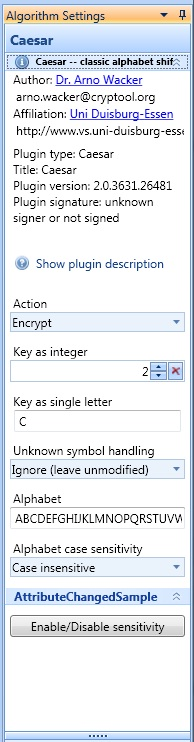
\includegraphics{figures/task_pane.jpg}
\end{center}

\begin{lstlisting}
using System;
using System.ComponentModel;
using System.Windows;
using System.Windows.Controls;

using Cryptool.PluginBase;

namespace Cryptool.Caesar
{
    public class CaesarSettings : ISettings
    {
        #region Public Caesar specific interface

        /// <summary>
        /// This delegate is ued to send log messages from
        /// the settings class to the Caesar plugin.
        /// </summary>
        public delegate void CaesarLogMessage(string msg, NotificationLevel loglevel);

        /// <summary>
        /// An enumeration for the different modes of handling
        /// unknown characters.
        /// </summary>
        public enum UnknownSymbolHandlingMode { Ignore = 0, Remove = 1, Replace = 2 };

        /// <summary>
        /// Fires when a new status message was sent.
        /// </summary>
        public event CaesarLogMessage LogMessage;

        public delegate void CaesarReExecute();

        public event CaesarReExecute ReExecute;

        /// <summary>
        /// Retrieves or sets the current shift value (i.e. the key).
        /// </summary>
        [PropertySaveOrder(0)]
        public int ShiftKey
        {
            get { return shiftValue; }
            set
            {
                setKeyByValue(value);
            }
        }

        /// <summary>
        /// Retrieves the current setting of whether or not the
        /// alphabet should be treated as case-sensitive.
        /// </summary>
        [PropertySaveOrder(1)]
        public bool CaseSensitiveAlphabet
        {
            get
            {
                if (caseSensitiveAlphabet == 0)
                {   return false;   }
                else
                {   return true;    }
            }
            set {} // this setting is readonly, but we must include
                   // some form of set method to prevent problems.
        }

        /// <summary>
        /// Returns true if any settings have been changed.
        /// This value should be set externally to false, i.e.
        /// when a project is saved.
        /// </summary>
        [PropertySaveOrder(3)]
        public bool HasChanges
        {
            get { return hasChanges; }
            set { hasChanges = value; }
        }

        #endregion

        #region Private variables
        private bool hasChanges;
        private int selectedAction = 0;
        private string upperAlphabet = "ABCDEFGHIJKLMNOPQRSTUVWXYZ";
        private string lowerAlphabet = "abcdefghijklmnopqrstuvwxyz";
        private string alphabet = "ABCDEFGHIJKLMNOPQRSTUVWXYZ";
        private char shiftChar = 'C';
        private int shiftValue = 2;
        private UnknownSymbolHandlingMode unknownSymbolHandling = UnknownSymbolHandlingMode.Ignore;
        private int caseSensitiveAlphabet = 0; // 0 = case-insensitve, 1 = case-sensitive
        private bool sensitivityEnabled = true;
        #endregion

        #region Private methods

        private string removeEqualChars(string value)
        {
            int length = value.Length;

            for (int i = 0; i < length; i++)
            {
                for (int j = i + 1; j < length; j++)
                {
                    if ((value[i] == value[j]) || (!CaseSensitiveAlphabet & (char.ToUpper(value[i]) == char.ToUpper(value[j]))))
                    {
                        LogMessage("Removing duplicate letter: \'" + value[j] + "\' from alphabet!", NotificationLevel.Warning);
                        value = value.Remove(j,1);
                        j--;
                        length--;
                    }
                }
            }

            return value;
        }

        /// <summary>
        /// Set the new shiftValue and the new shiftCharacter
        /// to offset % alphabet.Length.
        /// </summary>
        private void setKeyByValue(int offset)
        {
            HasChanges = true;

            // Make sure the shift value lies within the alphabet range.
            offset = offset % alphabet.Length;

            // Set the new shiftChar.
            shiftChar = alphabet[offset];

            // Set the new shiftValue.
            shiftValue = offset;

            // Announce this to the settings pane.
            OnPropertyChanged("ShiftValue");
            OnPropertyChanged("ShiftChar");

            // Print some info in the log.
            LogMessage("Accepted new shift value " + offset + "! (Adjusted shift character to \'" + shiftChar + "\')", NotificationLevel.Info);
        }

        private void setKeyByCharacter(string value)
        {
            try
            {
                int offset;
                if (this.CaseSensitiveAlphabet)
                {
                    offset = alphabet.IndexOf(value[0]);
                }
                else
                {
                    offset = alphabet.ToUpper().IndexOf(char.ToUpper(value[0]));
                }

                if (offset >= 0)
                {
                    HasChanges = true;
                    shiftValue = offset;
                    shiftChar = alphabet[shiftValue];
                    LogMessage("Accepted new shift character \'" + shiftChar + "\'! (Adjusted shift value to " + shiftValue + ")", NotificationLevel.Info);
                    OnPropertyChanged("ShiftValue");
                    OnPropertyChanged("ShiftChar");
                }
                else
                {
                    LogMessage("Bad input \"" + value + "\"! (Character not in alphabet!) Reverting to " + shiftChar.ToString() + "!", NotificationLevel.Error);
                }
            }
            catch (Exception e)
            {
                LogMessage("Bad input \"" + value + "\"! (" + e.Message + ") Reverting to " + shiftChar.ToString() + "!", NotificationLevel.Error);
            }
        }

        #endregion

        #region Algorithm settings properties (visible in the Settings pane)

        [PropertySaveOrder(4)]
        [ContextMenu("Action", "Select the algorithm action", 1, DisplayLevel.Beginner, ContextMenuControlType.ComboBox, new int[] { 1, 2 }, "Encrypt", "Decrypt")]
        [TaskPane("Action", "setAlgorithmActionDescription", null, 1, true, DisplayLevel.Beginner, ControlType.ComboBox, new string[] { "Encrypt", "Decrypt" })]
        public int Action
        {
            get
            {
                return this.selectedAction;
            }
            set
            {
                if(value != selectedAction)
                {
                	HasChanges = true;
	                this.selectedAction = value;
    	            OnPropertyChanged("Action");
    	        }
                if(ReExecute != null)
                {	ReExecute();	}
            }
        }

        [PropertySaveOrder(5)]
        [TaskPane("Key as integer", "Enter the number of letters to shift. For example, a value of 1 means that the plaintext character 'a' gets mapped to the ciphertext character 'B', 'b' to 'C', and so on.", null, 2, true, DisplayLevel.Beginner, ControlType.NumericUpDown, ValidationType.RangeInteger, 0, 100)]
        public int ShiftValue
        {
            get { return shiftValue; }
            set
            {
                setKeyByValue(value);
                if (ReExecute != null)
                {	ReExecute();	}
            }
        }

        [PropertySaveOrder(6)]
        [TaskPaneAttribute("Key as single letter", "Enter a single letter as the key. This letter is mapped to an integer stating the position in the alphabet. The values for 'Key as integer' and 'Key as single letter' are always synchronized.", null, 3, true, DisplayLevel.Beginner, ControlType.TextBox, ValidationType.RegEx, "^([A-Z]|[a-z]){1,1}")]
        public string ShiftChar
        {
            get { return this.shiftChar.ToString(); }
            set
            {
                setKeyByCharacter(value);
                if (ReExecute != null)
	                {   ReExecute();    }
            }
        }

        [PropertySaveOrder(7)]
        [ContextMenu("Unknown symbol handling", "What should be done with characters encountered in the input which are not in the alphabet?", 4, DisplayLevel.Expert, ContextMenuControlType.ComboBox, null, new string[] { "Ignore (leave unmodified)", "Remove", "Replace with \'?\'" })]
        [TaskPane("Unknown symbol handling", "What should be done with characters encountered in the input which are not in the alphabet?", null, 4, true, DisplayLevel.Expert, ControlType.ComboBox, new string[] { "Ignore (leave unmodified)", "Remove", "Replace with \'?\'" })]
        public int UnknownSymbolHandling
        {
            get { return (int)this.unknownSymbolHandling; }
            set
            {
                if((UnknownSymbolHandlingMode)value != unknownSymbolHandling)
                {
                	HasChanges = true;
	                this.unknownSymbolHandling = (UnknownSymbolHandlingMode)value;
    	            OnPropertyChanged("UnknownSymbolHandling");
				}
                if (ReExecute != null) 
                {	ReExecute();	}
            }
        }

        [SettingsFormat(0, "Normal", "Normal", "Black", "White", Orientation.Vertical)]
        [PropertySaveOrder(9)]
        [TaskPane("Alphabet", "This is the alphabet currently in use.", null, 6, true, DisplayLevel.Expert, ControlType.TextBox, "")]
        public string AlphabetSymbols
        {
          get { return this.alphabet; }
          set
          {
            string a = removeEqualChars(value);
            if (a.Length == 0) // cannot accept empty alphabets
            {
              LogMessage("Ignoring empty alphabet from user! Using previous alphabet instead: \" + alphabet + "\" (" + alphabet.Length.ToString() + " Symbols)", NotificationLevel.Info);
            }
            else if (!alphabet.Equals(a))
            {
              HasChanges = true;
              this.alphabet = a;
              setKeyByValue(shiftValue); // reevaluate if the shiftvalue is still within the range
              LogMessage("Accepted new alphabet from user: \"" + alphabet + "\" (" + alphabet.Length.ToString() + " Symbols)", NotificationLevel.Info);
              OnPropertyChanged("AlphabetSymbols");

              if (ReExecute != null)
              {	ReExecute();	}
            }
          }
        }

        /// <summary>
        /// Visible setting how to deal with alphabet case.
        /// 0 = case-insentive, 1 = case-sensitive
        /// </summary>
        [PropertySaveOrder(8)]
        [ContextMenu("Alphabet case sensitivity", "Should upper and lower case be treated as the same (so that 'a' = 'A')?", 7, DisplayLevel.Expert, ContextMenuControlType.ComboBox, null, new string[] { "Case insensitive", "Case sensitive" })]
        [TaskPane("Alphabet case sensitivity", "Should upper and lower case be treated as the same (so that 'a' = 'A')?", null, 7, true, DisplayLevel.Expert, ControlType.ComboBox, new string[] { "Case insensitive", "Case sensitive" })]
        public int AlphabetCase
        {
            get { return this.caseSensitiveAlphabet; }
            set
            {
                if (value != caseSensitiveAlphabet)
                {	HasChanges = true;	}
                this.caseSensitiveAlphabet = value;
                if (value == 0)
                {
                    if (alphabet == (upperAlphabet + lowerAlphabet))
                    {
                        alphabet = upperAlphabet;
                        LogMessage("Changing alphabet to: \"" + alphabet + "\" (" + alphabet.Length.ToString() + " Symbols)", NotificationLevel.Info);
                        OnPropertyChanged("AlphabetSymbols");
                        // reset the key (shiftvalue/shiftChar)
                        // to be in the range of the new alphabet.
                        setKeyByValue(shiftValue);
                    }
                }
                else
                {
                    if (alphabet == upperAlphabet)
                    {
                        alphabet = upperAlphabet + lowerAlphabet;
                        LogMessage("Changing alphabet to: \"" + alphabet + "\" (" + alphabet.Length.ToString() + " Symbols)", NotificationLevel.Info);
                        OnPropertyChanged("AlphabetSymbols");
                    }
                }

                // Remove equal characters from the current alphabet.
                string a = alphabet;
                alphabet = removeEqualChars(alphabet);
                if (a != alphabet)
                {
                    OnPropertyChanged("AlphabetSymbols");
                    LogMessage("Changing alphabet to: \"" + alphabet + "\" (" + alphabet.Length.ToString() + " Symbols)", NotificationLevel.Info);
                }
                OnPropertyChanged("AlphabetCase");
                if (ReExecute != null)
                {	ReExecute();	}
            }
        }

        #endregion

        #region INotifyPropertyChanged Members

        public event PropertyChangedEventHandler PropertyChanged;

        protected void OnPropertyChanged(string name)
        {
          if (PropertyChanged != null)
          {
            PropertyChanged(this, new PropertyChangedEventArgs(name));
          }
        }

        #endregion

        #region TaskPaneAttributeChanged (Sample)
        /// <summary>
        /// This event is here merely as a sample.
        /// </summary>
        public event TaskPaneAttributeChangedHandler TaskPaneAttributeChanged;

        [TaskPane("Enable/Disable sensitivity", "This setting is just a sample and shows how to enable / disable a setting.", "AttributeChangedSample", 8, false, DisplayLevel.Beginner, ControlType.Button)]
        public void EnableDisableSesitivity()
        {
          if (TaskPaneAttributeChanged!= null)
          {
            sensitivityEnabled = !sensitivityEnabled;
            if (sensitivityEnabled)
            {
              TaskPaneAttributeChanged(this, new TaskPaneAttributeChangedEventArgs(new TaskPaneAttribteContainer("AlphabetCase", Visibility.Visible)));
            }
            else
            {
              TaskPaneAttributeChanged(this, new TaskPaneAttributeChangedEventArgs(new TaskPaneAttribteContainer("AlphabetCase", Visibility.Collapsed)));
            }
          }
        }
        #endregion TaskPaneAttributeChanged (Sample)
    }
}
\end{lstlisting}